\subsubsection{Brushless Motoransteuerung}
\textbf{Theorie der Ansteuerung}:\\
\begin{wrapfigure}{r}{0.50\textwidth}
	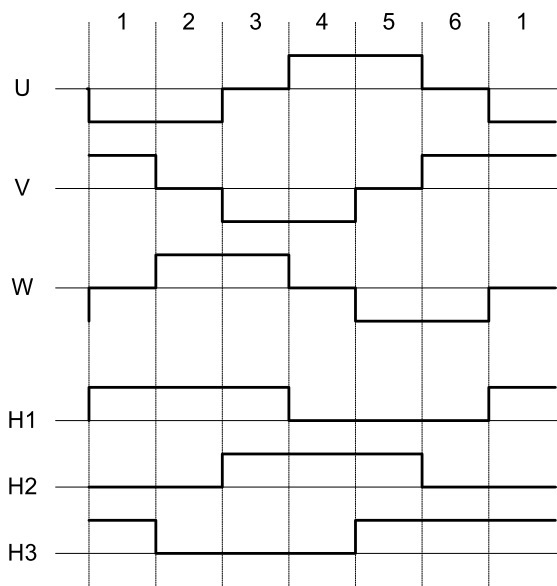
\includegraphics[scale=0.45]{\BrushlessPath/Bilder/ZeitlicheHallSensorAnsteuerung.jpg}
	\caption[Zeitliche Darstellung der Ansteuerung mit Hall-Sensoren]{Zeitliche Darstellung der Ansteuerung mit Hall-Sensoren \cite{AppNote:BrushlessuC}}
	\centering
    \label{abb:ZeitlicheAnsteuerungBrushlessMotor}
\end{wrapfigure}
Brushless-Motoren sind Synchron-Drehstrom-Motoren. Das heisst, sie werden mittels eines kontinuierlichen Drehfeld in Bewegung gesetzt. Dabei ist darauf zu achten, dass der Läufer dem Drehfeld synchron folgen kann, daher der Name. Falls der Läufer dem Drehfeld aus irgend einem Grund nicht folgen kann, so wird keine Spannung vom Rotor in die Statorwicklungen induziert, die der Erregerspannung entgegenwirkt. Daraus Folgt, dass ein immenser Strom fliesst, der nur von der Wicklungsimpedanz des Motors begrenzt wird.\\
Es gibt hauptsächlich zwei Methoden das Drehfeld zu regeln. Die eine und einfache Methode ist mittels drei Hallsensoren, die im Motor integriert sind. Dies macht den Motor aufwändiger und dementsprechend teurer. Die Regelung mit Hallsensoren ist verhältnismässig einfach, da je nach den Signalen die einzelnen Spulen direkt angesteuert werden kann. Der Zusammenhang zwischen der Ansteuerung und den Hall-Sensorsignalen ist in Abbildung \ref{abb:ZeitlicheAnsteuerungBrushlessMotor} ersichtlich. Dabei stehen $U$, $V$ und $W$ für die Phasenströme und $H_1$, $H_2$ und $H_3$ die entsprechenden Signale der Hallsensoren. Dieser Darstellung ist zu entnehmen, dass jedesmal wenn ein Hallsensor eine Änderung anzeigt, ein Nulldurchgang im entsprechenden Stromverlauf stattgefunden hat. Dies ist der Zeitpunkt, in dem die Kommutierung durchgeführt werden muss.
\\
\textbf{Aufbaubeschreibung}:
\begin{wrapfigure}{r}{0.55\textwidth}
	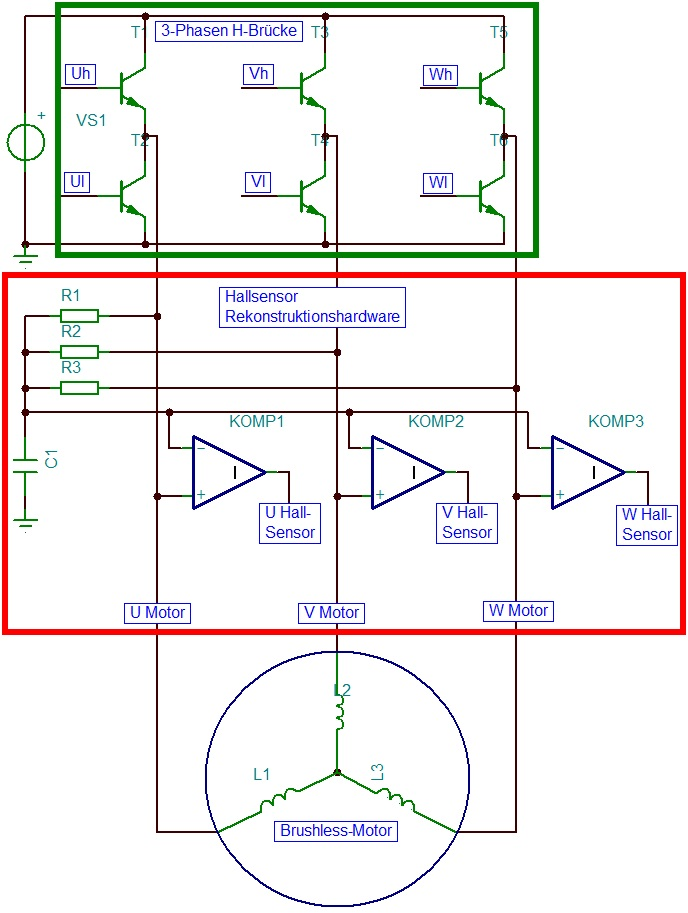
\includegraphics[scale=0.4]{\BrushlessPath/Bilder/MotoransteuerungSchema.jpg}
	\centering
	\caption{Schema des Brushless-Versuchsaufbaus}
\label{abb:MotoransteuerungSchema}
\end{wrapfigure}
Das Schema des gesamten Aufbaus des Tests ist in der Abbildung \ref{abb:MotoransteuerungSchema} abgebildet. Die 3-Phasen H-Brücke oben im grünen Rechteck wird direkt vom FPGA angesteuert. Die Hardware dieser Brücke ermöglicht eine voll galvanisch getrennte Ansteuerung mit 3.3V Logikpegeln. Diese Brücke wurde zur Verfügung gestellt und verwendet. Die Rekonstruktion der Hallsensoren-Signale findet im rot markierten Teil des Aufbaus statt. Dieser Part wurde auf einer Laborplatte aufgebaut und zusammen gelötet. Die so generierten Signale $U_{Hallsensor}$, $V_{Hallsensor}$, $W_{Hallsensor}$ werden einem FPGA geliefert. Anhand dieser Signale steuert dieses das FPGA die H-Brücken-Transistoren mittels der Signale $U_h$, $U_l$, $V_h$, $V_l$, $W_h$, $W_l$. Die im FPGA enthaltene Konfiguration sind simple AND-Verknüpfungen, die die anligenden Signale sehr schnell und effizient verarbeiten. Auf diese Weise ist es möglich, den Motor sehr schnell anzusteuern.\\
\\
In der Abbildung \ref{abb:MessplatzAufbau} ist der gesamte Aufbau abgebildet. Man beachte die markierten Felder. am unteren linken Rand ist der Motor befestigt. In der Mitte des Bildes ist die Hardware, mit der die Hallsensoren Signale rekonstruiert werden. Die generierten Signale werden dem FPGA in der unteren linken Ecke zugeführt. Diese Signale werden logisch verknüpft und danach werden die sechs Signale generiert um die H-Brücke in der oberen rechten Hälfte anzusteuern. Diese Wiederum treiben den Motor an.
\begin{figure}[h!]
%\vspace{-16pt}
	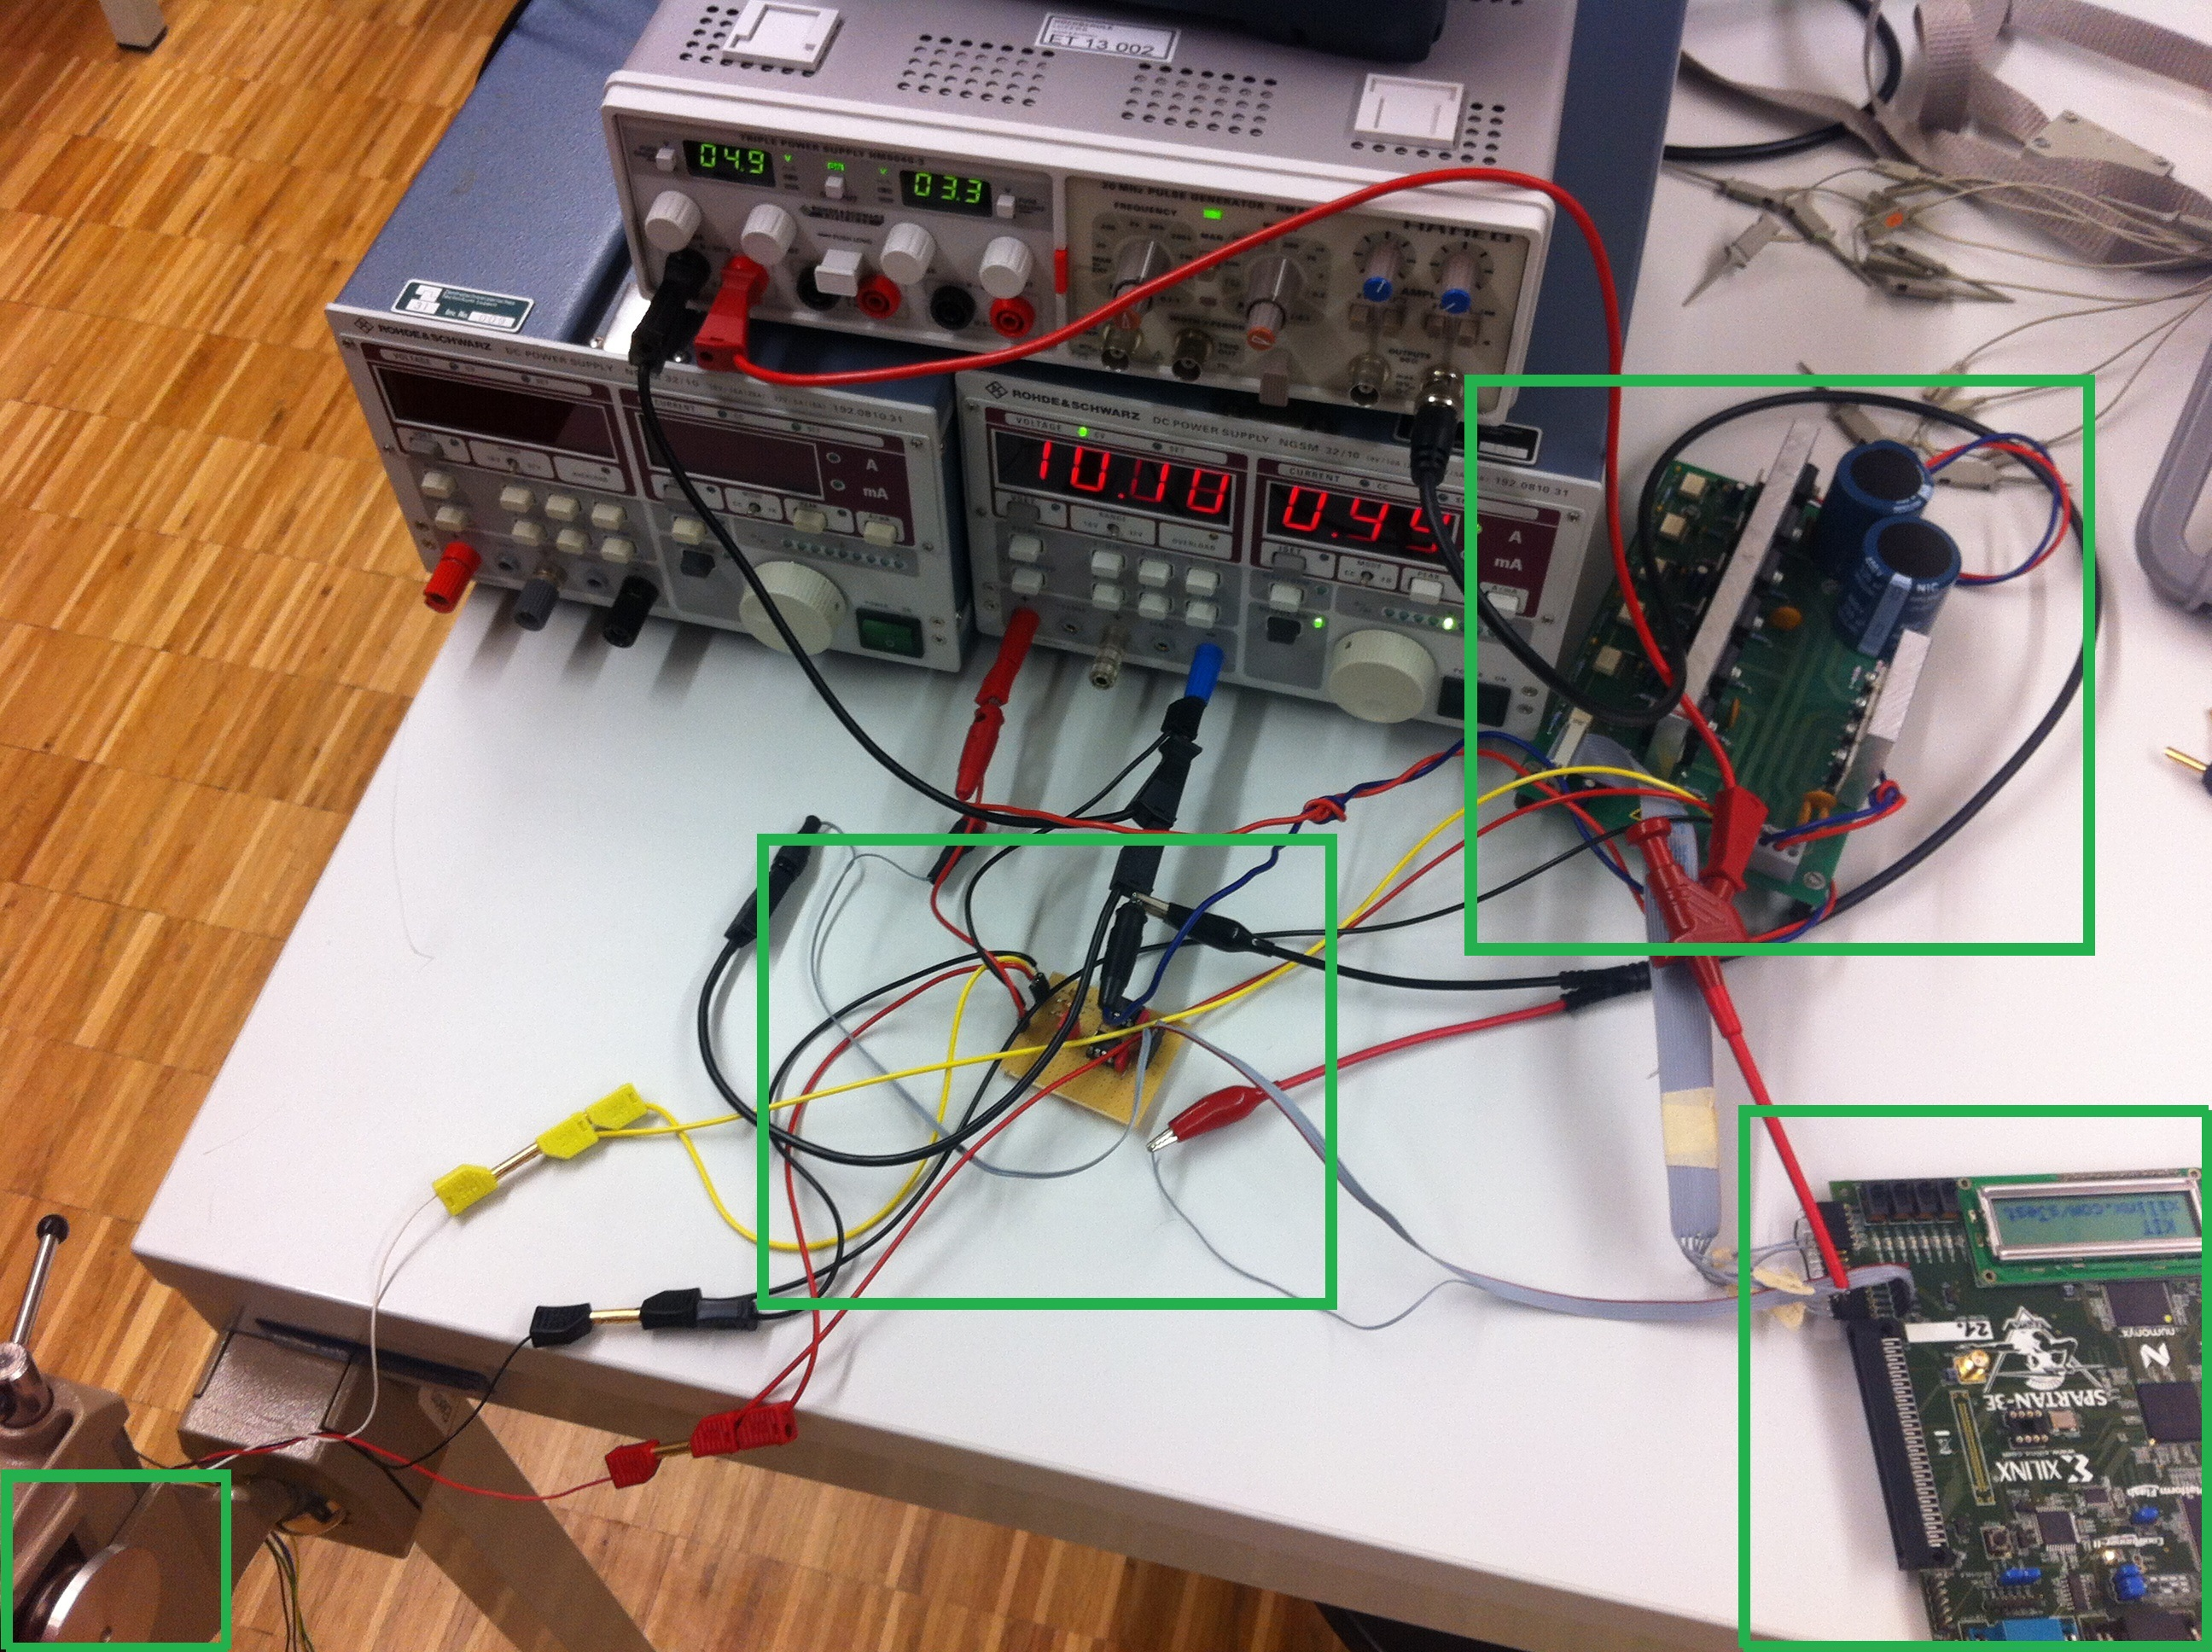
\includegraphics[scale=0.14]{\BrushlessPath/Bilder/MessplatzAufbau.jpg}
	\centering
	\caption{Testaufbau} 
\label{abb:MessplatzAufbau}
%\vspace{-10pt}
\end{figure}\\
Die im FPGA enthaltene Logik basiert auf der Wahrheitstabelle, die in Abbildung \ref{abb:WahrheitstabelleAnsteuerung} abgebildet ist.
\begin{figure}[h!]
\begin{tabular}{ccc||cc|cc|cc||c}
     $H_1$ & $H_2$ & $H_3$ & $U_h$ & $U_l$ & $V_h$ & $V_l$ & $W_h$ & $W_l$ & Illegal\\
\hline 0   &   0   &   0   &   0   &   0   &   0   &   0   &   0   &   0   &   1\\
       0   &   0   &   1   &   0   &   0   &   0   &   1   &   1   &   0   &   0\\
       0   &   1   &   0   &   0   &   1   &   1   &   0   &   0   &   0   &   0\\
       0   &   1   &   1   &   0   &   1   &   0   &   0   &   1   &   0   &   0\\
       1   &   0   &   0   &   1   &   1   &   0   &   0   &   1   &   0   &   0\\
       1   &   0   &   1   &   1   &   0   &   0   &   1   &   0   &   0   &   0\\
       1   &   1   &   0   &   0   &   0   &   1   &   0   &   0   &   1   &   0\\
       1   &   1   &   1   &   0   &   0   &   0   &   0   &   0   &   0   &   1\\
\end{tabular}
	\centering
	\caption{Wahrheitstabelle der Ansteuerung} 
\label{abb:WahrheitstabelleAnsteuerung}
\end{figure}\\
Die Tabelle kann pro Signal zu folgenden logischen Verknüpfung vereinfacht werden.\\
\begin{tabular}{ccc}
$U_h = H_1 \wedge \bar{H_2}$ & $V_h = H_2 \wedge \bar{H_3}$ & $W_h = \bar{H_1} \wedge H_3$\\
$U_l = \bar{H_1} \wedge H_2$ & $V_l = \bar{H_2} \wedge H_3$ & $W_l = H_1 \wedge \bar{H_3}$
\end{tabular}
